% Banner tiêu đề dự án
\noindent
\begin{tikzpicture}
  \node[anchor=west, inner sep=0pt] (textnode) at (72pt, 0) {%
    {\fontsize{11.5pt}{13pt}\selectfont\sffamily\bfseries\color{projectgreen}DỰ ÁN ỨNG DỤNG}%
    \hspace{7pt}{\color{black!40}\rule[-1.5pt]{0.8pt}{11pt}}\hspace{7pt}%
    {\fontsize{11.5pt}{13pt}\selectfont\sffamily\bfseries\color{black!90}GIẢI TÍCH VỀ CẦU VỒNG}%
  };
  \foreach \y in {-3.6pt, -1.8pt, 0pt, 1.8pt, 3.6pt} {
    \draw[projectgreen!75, line width=0.45pt] (0pt, \y) -- (66pt, \y);
    \draw[projectgreen!75, line width=0.45pt] ([xshift=7pt]textnode.east |- 0,\y) -- (\linewidth, \y);
  }
\end{tikzpicture}

\vspace{10pt}

% Đoạn giới thiệu đầu trang
\noindent\hfill
\begin{minipage}{0.69\textwidth}
  \fontsize{9.5pt}{12.5pt}\selectfont
  Cầu vồng được tạo ra khi các giọt nước mưa tán xạ ánh sáng mặt trời. Chúng đã mê hoặc nhân loại từ thời cổ đại và khơi nguồn cho những nỗ lực giải thích khoa học từ thời Aristotle. Trong dự án này, chúng ta sử dụng các ý tưởng của Descartes và Newton để giải thích hình dạng, vị trí và màu sắc của cầu vồng.
\end{minipage}

\vspace{12pt}

% Phần 1: Hình 1 và Bài toán 1
\noindent
\begin{minipage}[t]{0.28\textwidth}
  \vspace{0pt}
  \centering
  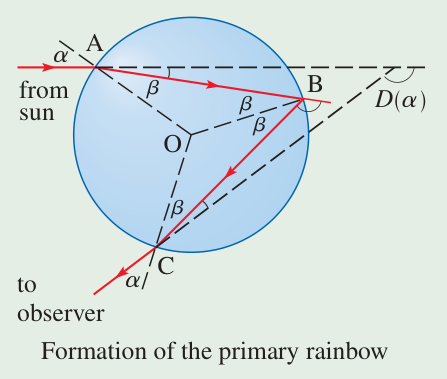
\includegraphics[width=\linewidth]{images/p0324_fig1.png}\\[4pt]
  {\fontsize{8.5pt}{10.5pt}\selectfont\sffamily Sự hình thành cầu vồng chính\par}
\end{minipage}%
\hfill
\begin{minipage}[t]{0.69\textwidth}
  \vspace{0pt}
  \fontsize{9.5pt}{12.5pt}\selectfont
  \textbf{1.}\enspace Hình vẽ bên cho thấy một tia sáng mặt trời đi vào một giọt nước mưa hình cầu tại $A$. Một phần ánh sáng bị phản xạ, nhưng đoạn thẳng $AB$ cho biết đường đi của phần ánh sáng đi vào bên trong giọt nước. Chú ý rằng tia sáng bị khúc xạ về phía pháp tuyến $AO$ và trên thực tế Định luật Snell cho biết $\sin\alpha = k\sin\beta$, trong đó $\alpha$ là góc tới, $\beta$ là góc khúc xạ, và $k \approx \frac{4}{3}$ là chiết suất của nước. Tại $B$, một phần ánh sáng truyền qua giọt nước và khúc xạ vào không khí, nhưng đoạn thẳng $BC$ cho biết phần ánh sáng bị phản xạ. (Góc tới bằng góc phản xạ.) Khi tia sáng tới $C$, một phần của nó bị phản xạ, nhưng hiện tại chúng ta quan tâm nhiều hơn đến phần rời khỏi giọt nước tại $C$. (Chú ý rằng nó bị khúc xạ ra xa pháp tuyến.) \textit{Góc lệch} $D(\alpha)$ là lượng góc quay theo chiều kim đồng hồ mà tia sáng đã trải qua trong quá trình gồm ba giai đoạn này. Do đó
  \[
  D(\alpha) = (\alpha - \beta) + (\pi - 2\beta) + (\alpha - \beta) = \pi + 2\alpha - 4\beta
  \]
  Hãy chứng minh rằng giá trị nhỏ nhất của góc lệch là $D(\alpha) \approx 138^\circ$ và xảy ra khi $\alpha \approx 59{,}4^\circ$.
\end{minipage}

\vspace{10pt}

% Phần 2: Hình 2, phân tích góc lệch và Bài toán 2
\noindent
\begin{minipage}[t]{0.28\textwidth}
  \vspace{0pt}
  \centering
  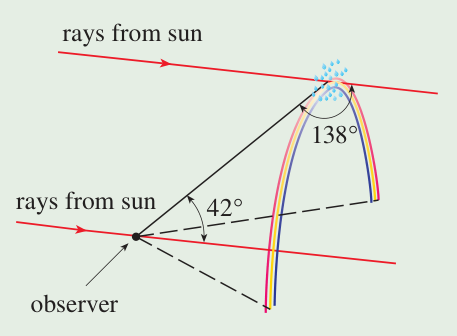
\includegraphics[width=\linewidth]{images/p0324_fig2.png}
\end{minipage}%
\hfill
\begin{minipage}[t]{0.69\textwidth}
  \vspace{0pt}
  \fontsize{9.5pt}{12.5pt}\selectfont
  \hspace*{1.5em}Ý nghĩa của góc lệch nhỏ nhất là khi $\alpha \approx 59{,}4^\circ$, ta có $D'(\alpha) \approx 0$, do đó $\Delta D / \Delta \alpha \approx 0$. Điều này có nghĩa là nhiều tia sáng có $\alpha \approx 59{,}4^\circ$ bị lệch đi xấp xỉ cùng một lượng như nhau. Chính sự \textit{tập trung} của các tia sáng đến từ gần hướng của góc lệch cực tiểu đã tạo nên độ sáng của cầu vồng chính. Hình bên trái cho thấy góc nâng từ người quan sát lên điểm cao nhất trên cầu vồng là $180^\circ - 138^\circ = 42^\circ$. (Góc này được gọi là \textit{góc cầu vồng}.)
  \par\vspace{8pt}
  \textbf{2.}\enspace Bài toán 1 giải thích vị trí của cầu vồng chính, nhưng làm thế nào để giải thích màu sắc của nó? Ánh sáng mặt trời bao gồm một dải các bước sóng, từ dải màu đỏ qua cam, vàng, lục, lam, chàm và tím. Như Newton đã khám phá trong các thí nghiệm với lăng kính vào năm 1666, chiết suất là khác nhau đối với mỗi màu sắc. (Hiện tượng này được gọi là sự \textit{tán sắc}.) Đối với ánh sáng đỏ, chiết suất là $k \approx 1{,}3318$, trong khi đối với ánh sáng tím là $k \approx 1{,}3435$. Bằng cách lặp lại phép tính ở Bài toán 1 cho các giá trị này của $k$, hãy chứng minh rằng góc cầu vồng là khoảng $42{,}3^\circ$ đối với dải màu đỏ và $40{,}6^\circ$ đối với dải màu tím. Vì vậy, cầu vồng thực sự bao gồm bảy cung riêng biệt tương ứng với bảy màu sắc.
\end{minipage}

\vspace{10pt}

% Phần 3: Hình 3 và Bài toán 3
\noindent
\begin{minipage}[t]{0.28\textwidth}
  \vspace{0pt}
  \centering
  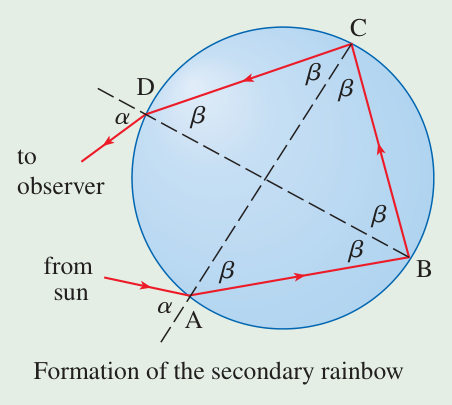
\includegraphics[width=\linewidth]{images/p0324_fig3.png}\\[4pt]
  {\fontsize{8.5pt}{10.5pt}\selectfont\sffamily Sự hình thành cầu vồng phụ\par}
\end{minipage}%
\hfill
\begin{minipage}[t]{0.69\textwidth}
  \vspace{0pt}
  \fontsize{9.5pt}{12.5pt}\selectfont
  \textbf{3.}\enspace Có lẽ bạn đã từng nhìn thấy một cầu vồng phụ mờ hơn ở phía trên cầu vồng chính. Hiện tượng đó xuất phát từ phần tia sáng đi vào một giọt nước mưa và bị khúc xạ tại $A$, phản xạ hai lần (tại $B$ và $C$), rồi khúc xạ khi nó rời khỏi giọt nước tại $D$ (xem hình bên trái). Lần này góc lệch $D(\alpha)$ là tổng lượng góc quay ngược chiều kim đồng hồ mà tia sáng trải qua trong quá trình bốn giai đoạn này. Hãy chứng minh rằng
  \[
  D(\alpha) = 2\alpha - 6\beta + 2\pi
  \]
  và $D(\alpha)$ đạt giá trị nhỏ nhất khi
  \[
  \cos\alpha = \sqrt{\frac{k^2 - 1}{8}}
  \]
  \par\vspace{10pt}
  \hfill \textit{(còn tiếp)}
\end{minipage}
